The lead shield and the active vetos were included in the simulation of TRITIUM-IFIC-2 to quantify the reduction of cosmic background detected. A flat cosmic ray source of $1 \times 1~\meter^2$ placed at a height of $70~\cm$ was simulated with the cosmic ray generator of the CRY library. Two R8520-460 PMTs from Hamamatsu were simulated to read each plastic scintillator out, as described in section \ref{sec:IntroductionBackground}. The lead shield was simulated with the lead properties taken from the Geant4 NIST database. The dimensions of the simulated lead shield were $60 \times 60 \times 70~\cm^3$, suitable for one TRITIUM-IFIC-2 prototype and an active cosmic veto. These dimensions were set smaller than the real dimension of the lead shield at Arrocampo to save computing time and resources. Energy, position and momentum distribution were produced. Simulations with three different shielding configurations were carried out with the aim of quantifying the background rejection due to the passive shield and the active veto. The first configuration consisted of one TRITIUM-IFIC-2 prototype and the cosmic ray source. In the second configuration, a lead shield was added and in the third one the cosmic veto was also included. The cosmic events detected by TRITIUM-IFIC-2 are shown in Figure \ref{fig:CosmicEventsSuppressionSimulated}, for the three configurations. Cosmic rays detected by TRITIUM-IFIC-2 are reduced by a factor around 5.5 when a lead shield $5~\cm$ thick is included (this is the width of the shield currently installed at Arrocampo). This reduction is caused by the suppression of the soft cosmic radiation (energy lower than $200~\MeV$). The natural background of the installation site, which would be also mitigated by the lead shield, was not included in this simulation. Therefore, the expected background reduction due to the passive veto would be even better. Around $60\%$ of the cosmic rays that penetrate the lead shield and reach TRITIUM-IFIC-2 are mostly hard cosmic rays which are detected by the cosmic veto and suppressed from the background. In summary, cosmic rays that would be detected and misidentified as tritium electrons by TRITIUM-IFIC-2 are reduced by $92.6\%$ by the background rejection system. Since the natural background of the site was not included in the simulations, the actual background reduction is expected to be even larger.

\begin{figure}[h]
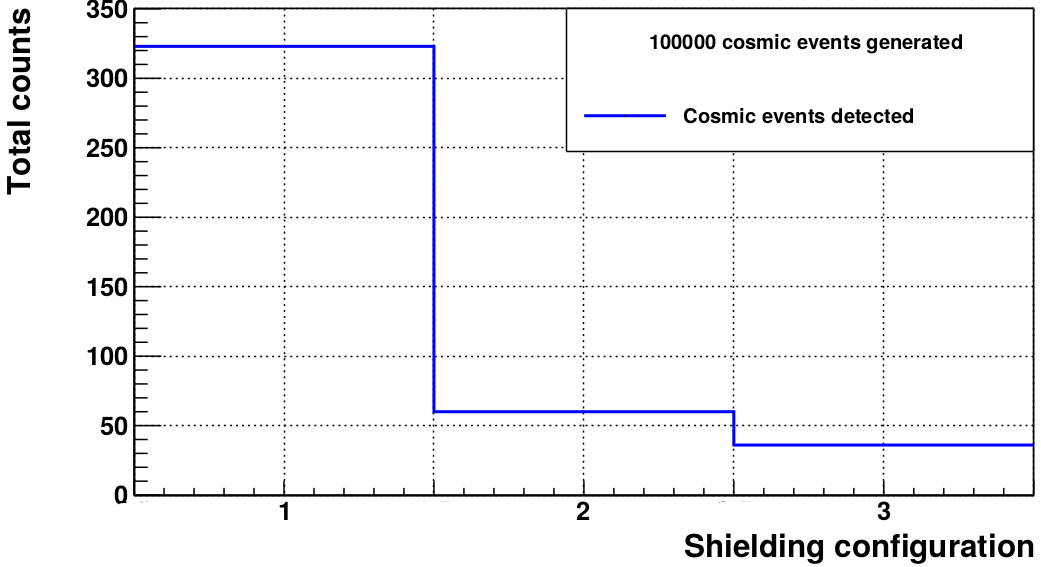
\includegraphics[scale=0.35]{6Simulations/62TRITIUMMonitor/622BackgroundRejectionSystem/Suppression_of_cosmic_events.png}
\centering
\caption{Cosmic ray events detected and misidentified as tritium events by TRITIUM-IFIC-2 from $10^5$ generated cosmic rays for the three different shielding configurations. Bin 1 corresponds to the absence of the background rejection system. Bin 2 corresponds to the passive shield and bin 3 corresponds to both lead shield and cosmic veto.  \label{fig:CosmicEventsSuppressionSimulated}}
\end{figure}